\documentclass[11pt]{article}
\usepackage[margin=1in]{geometry}
\usepackage[T1]{fontenc}
\usepackage{lmodern,amsmath,amssymb,booktabs,graphicx,hyperref}
\hypersetup{colorlinks=true,linkcolor=blue,citecolor=blue,urlcolor=blue}
\setlength{\emergencystretch}{2em}
\newcommand{\ScalarIntervals}{370}
\newcommand{\ScalarNodes}{371}
\newcommand{\ScalarMaximum}{8.405509181456809}
\newcommand{\ScalarOwner}{370}
\newcommand{\ScalarLocalMaximum}{0.08778167488957692}

\newcommand{\PhotonCompleteRatio}{0.590609601653}
\newcommand{\PhotonDerivativeRatio}{0.908932991228}
\newcommand{\PhotonShellKernel}{0.428281024643}

\title{Berger--Hopf Standard Model:\\Action-domain localization and an auditable route to physical predictions}
\author{Norman P. Carberry\\Independent Researcher\\
\href{https://orcid.org/0009-0000-6650-3485}{ORCID: 0009-0000-6650-3485}}
\date{Working manuscript, 7 September 2026}
\begin{document}
\maketitle
\begin{center}
\small\textbf{Research draft. Physical completion and journal submission remain open.}
\end{center}

\begin{abstract}
The Berger--Hopf Standard Model (BHSM) investigates whether a common
stratified variational framework can organize Standard Model-associated
structure without using measured masses or mixing angles to choose its
upstream dynamics. We formulate the current evidence boundary around
action-domain localization, finite-history response, and the transfer from
certified mathematical objects to physical observables. The authorized AE3
extension promotes a retained reciprocal-join profile to a response
constraint, yielding a regular local material carrier without a new
continuous coefficient. Separately, a 512-bit interval calculation composes
the frozen central scalar response across \ScalarIntervals{} intervals and
\ScalarNodes{} nodes, with maximum response-norm upper bound
\(\ScalarMaximum\). We describe the complete ambient midpoint chain rule
required for the remaining signed transverse calculation and an explicit
bound on stored coordinate-solve error. A separate photon audit corrects a
finite-mode symmetry diagnostic while retaining a positive-energy obstruction
on the reference Maxwell shell. We also distinguish a stationary
Einstein--Cartan domain rejection and a conditional charged-lepton tree
sum rule from a physical mass prediction. These results do not establish the
joint physical background, particle masses, mixing matrices, scattering
observables, or full BHSM completion. The manuscript binds numerical values
to immutable source artifacts and identifies the remaining proof operands
that must precede a physical prediction.
\end{abstract}

\section{Scientific scope and provenance}
BHSM is an evolving mathematical and computational research program.
Its historical spectral and coupling screens, conditional structural
results, numerical center calculations, and outward certificates have
different logical authority. A numerical match cannot close a missing
action, domain, normalization, or observable map. The present draft therefore
organizes results by their actual hypotheses and reproducible evidence,
rather than treating an earlier release label as physical completion.

The current definition of done requires every claimed quantity to share one
declared parent action and input ledger, with the intervening variational,
operator, scale, and observable maps closed \cite{status,dod}. Measured mass
and mixing data may enter a later comparison; they may not select a branch,
coefficient, normalization, regularization, or eigenvector ordering upstream.
Frozen historical outputs remain unchanged and retain their original labels.

This manuscript is the working source for the current flagship synthesis.
It reports completed local results and a precisely delimited computational
frontier. It is not a submission-ready claim of a complete physical model.

\section{Stratified action and physical ownership}
The retained architecture distinguishes a provisional \(S^8\) parent,
a relative two-cap \(S^{5|4}\) construction, and an intrinsic localized
four-dimensional effective theory. Compatibility maps between these strata
are part of the model specification. Fields, coefficients, and domains
cannot be moved between strata without an explicit action-owned map.

At the current finite-history frontier, geometry-local derivative kernels
are necessary computational inputs. They are not by themselves the complete
gauge, ghost, fermion, scalar, and mixed-field derivatives of one physical
background. Similarly, an implemented spectrum, vertex, or collision engine
does not supply the action-derived operands that it is designed to consume.
These distinctions prevent a software capability from being counted as a
physical prediction \cite{status,dod}.

The current program combines compatible local pieces as they become
available. A composed claim is permitted only when its pieces share the
action version, background, domain, scale and renormalization conventions,
and provenance chain. Later candidate action representatives are not
silently identified with an earlier certified representative.

\section{The AE3 local material carrier}
\subsection{Response constraint}
The retained reciprocal-join profile is
\begin{equation}
 \sigma_0(\chi)=-\frac12+\frac{2\chi}{\pi}
                    -\frac{\sin(4\chi)}{2\pi},
 \qquad 0\leq\chi\leq\frac\pi2.
\end{equation}
AE3 promotes this previously fixed profile into the existing eta-to-sigma
response constraint. On the oriented orbit space \(Q\), define
\begin{equation}
 W_J[\eta]=\sin^2f\cos^2f,\qquad
 Z_J[\eta]=\int_Q W_J[\eta]\,d\ell,
\end{equation}
and impose
\begin{equation}
 C_\sigma=n_\eta^A\nabla_A\sigma-\frac{W_J[\eta]}{Z_J[\eta]}=0,
 \qquad \sigma|_{Q_-}=-\frac12.
\end{equation}
The nonpropagating multiplier \(\lambda_\sigma\) supplies the response term
\begin{equation}
 S_{\rm response}=\int dt\int_Q d\ell\,\mu_Q\lambda_\sigma C_\sigma.
\end{equation}
The corresponding action replaces the old fixed profile wherever it occurs
and adds this constraint once. It does not add the retained Hopf/FR energy a
second time. This authorized action-domain promotion introduces no new
continuous coefficient, physical scale, or particle label \cite{ae3}.

\subsection{Regularity and scope}
On the retained identity branch,
\begin{equation}
 \sigma_0'(\chi)=\frac4\pi\sin^2(2\chi)>0
 \quad(0<\chi<\pi/2),\qquad
 \sigma_0(\pi/4)=0,\quad \sigma_0'(\pi/4)=\frac4\pi.
\end{equation}
Thus the material zero is transverse. The local carrier is
\begin{equation}
 D_{\rm enc}=\{\sigma<0\},\qquad
 \Sigma_{\rm enc}=\{\sigma=0\},\qquad
 n=\frac{\nabla\sigma}{|\nabla\sigma|}.
\end{equation}
The retained weight \(\Lambda(\sigma)=1-4\sigma^2\) is the unique even
polynomial of degree at most two with unit value at the seam and zeros at
\(\sigma=\pm1/2\). The associated boundary and flux cancellation statements
refer to this smooth internal material interface. The event-time condition
and the material surface are distinct objects.

The current algebraic transport retains three charged sectors and three
family slots. The resulting nine fibers preserve their supplied BHSM state
labels through the carrier construction; the geometry does not independently
select a particle species. This does not establish commutation with the
still-missing interacting history Hamiltonian or a persistent full-field
particle \cite{status}. The older unchanged-AE2 audit, in which none of six
candidate carriers qualified, remains a valid historical result within AE2.

\section{Complete finite-history second variation}
\subsection{Why the midpoint requires the full ambient space}
Let \(E\) be the 99-by-74 augmented trial frame, \(e\) its current-Green
coordinate axis, and \(V\) the stored 74-by-73 transverse basis. The retained
midpoint tensor contains \(H[U,U]\), where \(U=EV\) and \(H=D^2F\).
Transverse endpoint variations need not remain transverse at a
Hermite--Simpson midpoint. They can acquire axis and frame-normal components.
Dropping those terms is not justified by a small binary64 residual.

For fixed interval length \(h_i\), the endpoint-pair midpoint map has blocks
\begin{align}
 M_L&=\tfrac12E_iP_i+\tfrac{h_i}{8}DF_iE_iP_i,\\
 M_R&=\tfrac12E_{i+1}P_{i+1}-\tfrac{h_i}{8}DF_{i+1}E_{i+1}P_{i+1}.
\end{align}
The fixed reset has zero left variation at interval zero. Complete the
actual retained directions to a square ambient basis \(S=[U\ C]\), with
26 complement columns, and solve
\begin{equation}
 M=[M_L\ M_R]=UA+CD.
\end{equation}
For each output component, the full pullback is
\begin{equation}\label{eq:fullpullback}
 H[M,M]=A^TQ_{UU}A+A^TQ_{UC}D
       +D^TQ_{UC}^TA+D^TQ_{CC}D.
\end{equation}
Both cross terms and the complement-complement block are required. Their
signs may reinforce or cancel the retained contribution. An incomplete
transverse-only norm is neither an upper nor a lower bound for the full
pullback \cite{signed}.

\subsection{Signed assembly before norms}
Writing \(\mathcal A_i=-R_i^{-1}E_{i+1}^T\) for the unchanged reduced solve
and test-frame map, the local second response is
\begin{align}
 \mathcal S_i={}&\left(\frac{h_i}{6}\mathcal A_i
              +\frac{h_i^2}{12}\mathcal A_iDF_{i+1/2}\right)B_i\nonumber\\
 &+\frac{2h_i}{3}\mathcal A_iH_{i+1/2}[M_i,M_i]\nonumber\\
 &+\left(\frac{h_i}{6}\mathcal A_i
              -\frac{h_i^2}{12}\mathcal A_iDF_{i+1/2}\right)B_{i+1}.
\end{align}
All tensors are first pulled back to the common endpoint-pair coordinates.
The midpoint incidence terms retain their signs. If a local block is \(T\)
and a causal transport is \(P\), the identity
\begin{equation}
 \|PT\|_F^2=\operatorname{tr}(P TT^T P^T)
\end{equation}
retains output covariance through the transport. Contributions from adjacent
intervals acting on the same global diagonal input block must also be added
with their signed cross covariance before taking a norm. The existing
block-sup proof domain supplies the remaining triangle inequalities.

\subsection{Stored-basis and coordinate-solve verification}
Binary64 center assembly is distinct from an outward enclosure. For an exact
stored binary64 basis \(S\), a 512-bit Arb inverse enclosure verifies
nonsingularity without deleting a small singular direction. If \(\widehat X\)
is a computed coordinate matrix and \(M\) the exact stored binary64 target,
\begin{equation}\label{eq:solveerror}
 \|S^{-1}M-\widehat X\|_\infty
 \leq \|S^{-1}\|_\infty\,\|M-S\widehat X\|_\infty.
\end{equation}
Arb supplies the residual and inverse bounds \cite{arb,solve}. Equation
\eqref{eq:solveerror} controls this stored solve only. Physical direction
construction, Hessian rounding, propagation of coordinate error through
\eqref{eq:fullpullback}, and the action-neighborhood remainder are separate
required operands.

\section{Verified numerical evidence}
The completed correlated scalar calculation uses 512-bit interval arithmetic
and the frozen causal frames and preconditioner. Table~\ref{tab:scalar} and
Figure~\ref{fig:scalar} are generated from the source certificate after its
NPZ data hash is verified \cite{scalar}. No values are fitted to experimental
particle data.
\begin{table}[ht]
\centering
\caption{Completed frozen central scalar calculation. These are scoped
mathematical bounds, not physical mass or scattering observables.}
\label{tab:scalar}
\begin{tabular}{lr}
\toprule
Quantity & Recorded result\\
\midrule
Intervals / nodes & \ScalarIntervals{} / \ScalarNodes{}\\
Arithmetic precision & 512 bits\\
Maximum causal response norm upper & \ScalarMaximum\\
Node owning the maximum & \ScalarOwner\\
Maximum local second-residual norm upper & \ScalarLocalMaximum\\
\bottomrule
\end{tabular}
\end{table}
\begin{figure}[ht]
\centering
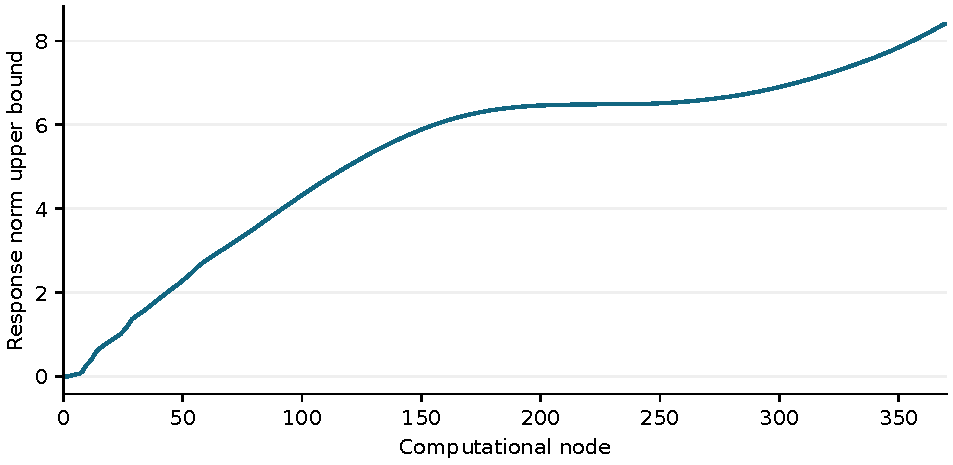
\includegraphics[width=\linewidth]{generated/scalar_response.pdf}
\caption{Actual certified numerical response along the frozen path. The
horizontal coordinate is a computational node index, not laboratory time.
The vertical value is a response-norm upper bound. The central scalar
certificate does not enclose the complete transverse neighborhood.}
\label{fig:scalar}
\end{figure}

The signed tensor recovery requires 370 endpoints and 370 midpoints. At each
midpoint the 26 complement directions require \(73\cdot26+26\cdot27/2=2249\)
new directional pairs, in addition to the retained symmetric transverse
block. These are contraction counts, not empirical CPU estimates. At this
draft's evidence boundary, the recovery and supplemental campaign are still
in progress; no complete signed center coefficient or outward two-radius
certificate is reported here.

\section{Photon diagnostic and the retained frozen route}
Write the retained dimensionless transverse Dirichlet-to-Neumann kernel as
\(N(s,q^2)\), with coexact \(s=n^2\), \(n\geq2\), and
\(q^2=(\omega R_4)^2\). For the normalized regular extension
\(u(\pi/2)=1\), put \(p=W\sin\rho\), \(m=W/\sin\rho\), where
\(W=1-4\sigma^2\), \(\sigma(\rho)=\sigma_0(\rho/2)\), is positive
in the interior. The stationary energy is
\begin{equation}
 N(s,q^2)=\int_0^{\pi/2}\bigl[p(u')^2+(s m-q^2p)u^2\bigr]\,d\rho.
\end{equation}
The regular endpoint makes the integration-by-parts term vanish.
At zero frequency, let \(T=\int p u^2\), \(M=\int m u^2\), and
\(G=\int p(u')^2\). The variational identities give
\begin{equation}
 -\partial_{q^2}N=T,\qquad \partial_sN=M,\qquad N(s,0)=G+sM.
\end{equation}
The earlier complete-mode ratio \(sT/N(s,0)\) is therefore distinct from
the spectral-derivative ratio \(T/M\). At \(n=2\), an independent
Riccati/sensitivity calculation gives \(\PhotonCompleteRatio\) and
\(\PhotonDerivativeRatio\), respectively \cite{photon}. These are binary64
witnesses checked against the retained solver, energy integrals, parameter
differences, and cutoff halving; they are not outward enclosures.

The first ratio tests an exact whole-kernel identification with
\(Z(s-q^2)\), but is not a universal Lorentz-symmetry test for a nonlocal
operator. The flat decaying half-space control \(N=\sqrt{s-q^2}\) has
complete-mode ratio \(1/2\) and derivative ratio one. Square-root
Dirichlet-to-Neumann operators are standard \cite{extension}. Freezing the
retained wall coefficients gives that same formal order-one principal
symbol on the spacelike branch. This does not construct a global causal
quantum propagator or control the null/glancing limit.

A direct obstruction remains on the reference Maxwell shell:
\begin{equation}
 N(s,s)=\int_0^{\pi/2}\bigl[p(u')^2+s(m-p)u^2\bigr]\,d\rho>0.
\end{equation}
The normalized trace is nonzero and \(m-p>0\) in the interior. At the
lowest mode, \(N(4,4)=\PhotonShellKernel\). The isolated frozen kernel
has no zero, and its inverse has no pole, on this shell; reflection doubles
the positive kernel. This rejects the specified frozen Maxwell route. It
does not exclude every completion or establish a global violation of local
Lorentz symmetry. Neither diagnostic ratio is a measured speed of light.

\section{Stationary domain and conditional flavor evidence}
\subsection{The Einstein--Cartan candidate}
The retained nonzero spin-source mode has
\(J=\sin^3(2\chi)\), \(u_0=N_0J^{-1/2}\sin\chi\), and
\(\Lambda\sim64\chi^3/(3\pi)\). Its ordinary norm is finite, but
\begin{equation}
 \frac{\sin^4\chi}{J\Lambda}
 =\frac{3\pi}{512}\chi^{-2}+O(1).
\end{equation}
This obstruction survives in the uneliminated projected action
\(\int(AK^2/2+SK)\,d\chi\). Compactly supported interior variations
require \(K_*=-S/A\), with \(A=O(\chi^6)\), \(S=O(\chi^2)\).
The stationary total is \(-S^2/(2A)\sim-c\chi^{-2}\), \(c>0\): its quadratic
and linear divergences do not cancel. An endpoint condition cannot change
that unique interior algebraic solution \cite{dependencyaudit}.

For a nonzero pure power-law source mode \(u\sim c\chi^\beta\),
ordinary normalizability requires \(\beta>-2\), while this EC form
requires \(\beta>-1/4\). The retained \(\beta=-1/2\) fails the latter.
The result rejects this candidate on the retained mode; it does not repair
the action or exclude different backgrounds or vanishing spin sources.

\subsection{The lepton relation and its missing dressing}
For the admitted heavy, middle, and light charged-lepton slots,
\((K,q^2)=(0,0),(35,1),(99,9)\), the retained family formula is
\begin{equation}
 m_f=M_{\rm common}\exp\!\left[-\frac{K_f+(a^2-1)q_f^2}{4\pi}\right].
\end{equation}
Eliminating the common scale and squashing gives the exact conditional
tree relation
\begin{equation}
 R_{\rm tree}=\log\frac{m_e}{m_\tau}
             -9\log\frac{m_\mu}{m_\tau}-\frac{54}{\pi}=0.
\end{equation}
This algebra does not independently select the supplied ledger.
For positive dressed masses \(M_f=Z_fm_f\), direct substitution gives
\begin{equation}
 R_{\rm pole}=\log Z_e-9\log Z_\mu+8\log Z_\tau,
 \qquad D=e^{R_{\rm pole}}=\frac{Z_eZ_\tau^8}{Z_\mu^9}.
\end{equation}
The stored post-derivation comparison requires \(D\simeq1.06056689915\).
It is not an input for choosing a self-energy. A common multiplicative
rescaling cancels, but additive or nondiagonal corrections are not excluded.
The physical calculation of \(D\) and its uncertainty remains open
\cite{dependencyaudit}.

The family-resolved first-order lepton operator and reset-glued domain
already exist. Advanced and retarded Green operators exist on each
finite-core globally hyperbolic history; this uses established causal
operator theory \cite{baer}. It does not select the physical history or
Feynman state, evaluate a dressed kernel, or define a global frequency pole
on a time-dependent history. The quark response additionally lacks its
action-owned up/down vertex normalizations and the left-handed embedding
dressing needed for nontrivial physical mixing. These gaps remain distinct
from the numerical response campaign.

\section{Physical observables and remaining obligations}
The project's physical finish line is stronger than successful local
certificates. It requires the complete joint finite-history operator oracle,
projected heat-minus-zeta force, KKT root, and constrained physical Hessian,
together with compatible downstream maps and continuum control. A positive
center screen alone cannot establish these objects.

Every claimed observable must eventually be classified once as a derived
point prediction, interval prediction, selection rule, qualitative structure,
comparison only, open internal blocker, or outside BHSM 1.0 scope
\cite{dod}. The required coverage includes the universal electromagnetic
vertex and muon magnetic moment; stability and decays; spectral enclosures
or exclusions; the known-particle inventory; and representative QED, weak,
strong, scalar, flavor, and neutrino scattering benchmarks. This draft
does not substitute a list of implemented engines for that completed matrix.

The minimal Standard Model and any effective neutrino extension must remain
distinguished. No confinement theorem, completed no-extra-light-state
theorem, or first-principles derivation of all Standard Model data is asserted.
A failed numerical representation screen also does not prove physical
instability or nonexistence of a root.

\section{Reproduction, data availability, and manuscript status}
The plotted values and the table are generated from the immutable scalar
source at revision \texttt{d75e77bb}; the downloadable Museum dataset records
the full 40-character revision and source SHA-256 digests. The exporter
refuses an unvalidated certificate, a changed data hash, a mismatch with
the recorded source revision, or an inconsistent array shape or maximum.
The plotting generator consumes the same dataset. Repeated artifact
materializations are compared byte for byte.

The complete scientific source and claim ledgers are available in the
repository \cite{repo}. This draft is maintained separately from frozen
historical manuscripts. Its abstract, results, and conclusions must be
updated from completed certificates before external submission; pending
physical quantities are not represented by simulated replacement values.

Computational and editorial work used Codex assistance. The scientific
provenance is the repository's retained action, derivations, tests, and
certificates. Author declarations, venue-specific formatting, and the final
scientific review remain part of submission preparation. No journal
submission or acceptance is claimed.

\begin{thebibliography}{99}
\raggedright
\bibitem{repo} N. P. Carberry, \emph{Berger--Hopf Standard Model research
repository}, \url{https://github.com/ncarberry64/Berger-Hopf-Standard-Model}.
\bibitem{status} N. P. Carberry, \emph{Current BHSM status}, repository
revision \texttt{d75e77bb}, \texttt{docs/current\_bhsm\_status.md}.
\bibitem{dod} N. P. Carberry, \emph{BHSM 1.0 definition of done}, same
revision, \texttt{docs/BHSM\_1\_0\_DEFINITION\_OF\_DONE.md}.
\bibitem{ae3} N. P. Carberry, \emph{BHSM-AE-3 reciprocal-join localization
and enclosure theorem}, same revision,
\texttt{theory/ae3\_reciprocal\_join\_localization\_enclosure.md}.
\bibitem{signed} N. P. Carberry, \emph{Current-Green signed transverse
causal center}, same revision,
\texttt{theory/n12\_gate7\_current\_green\_signed\_transverse\_causal\_center.md}.
\bibitem{scalar} N. P. Carberry, \emph{Current-Green correlated central
scalar causal composition certificate}, same revision, artifact
\texttt{BHSM\_N12\_GATE7\_CURRENT\_GREEN\_CORRELATED\_SCALAR\_CAUSAL\_COMPOSITION}.
\bibitem{solve} N. P. Carberry, \emph{Stored midpoint coordinate solve
certificate}, same revision, script
\texttt{certify\_n12\_gate7\_current\_green\_midpoint\_coordinate\_solve.py}.
\bibitem{arb} F. Johansson, ``Arb: Efficient arbitrary-precision
midpoint-radius interval arithmetic,'' \emph{IEEE Transactions on Computers}
\textbf{66}(8), 1281--1292 (2017).
\href{https://doi.org/10.1109/TC.2017.2690633}{doi:10.1109/TC.2017.2690633};
\url{https://arxiv.org/abs/1611.02831}.
\bibitem{photon} N. P. Carberry, \emph{AE3 photon diagnostic scope audit},
repository revision \texttt{016aa4b4},
\href{https://github.com/ncarberry64/Berger-Hopf-Standard-Model/blob/016aa4b48a87dcb53cdf50a05e9010d9777d208c/theory/ae3_c2_photon_symbol_audit.md}{derivation and numerical report}.
\bibitem{dependencyaudit} N. P. Carberry, \emph{BHSM mass and mixing
dependency audit}, repository revision \texttt{1ad740b5},
\href{https://github.com/ncarberry64/Berger-Hopf-Standard-Model/blob/1ad740b5ada806e3c5845a379c62d7f29712c6ff/docs/BHSM_MASS_MIXING_DEPENDENCY_AUDIT_2026_09_07.md}{action-domain audit and linked flavor derivations}.
\bibitem{extension} M. Kwa\'snicki and J. Mucha, \emph{Extension technique
for complete Bernstein functions of the Laplace operator} (2017),
\url{https://arxiv.org/abs/1707.02475}.
\bibitem{baer} C. B\"ar, ``Green-hyperbolic operators on globally hyperbolic
spacetimes,'' \emph{Communications in Mathematical Physics} \textbf{333},
1585--1615 (2015), \url{https://arxiv.org/abs/1310.0738}.
\end{thebibliography}
\end{document}
